\documentclass[submission]{eptcs}
\providecommand{\event}{TTC 2014}

\usepackage[T1]{fontenc}
\usepackage{url}
\usepackage{hyperref}
\usepackage[cache]{minted}
\newminted{clojure}{fontsize=\fontsize{8}{8},linenos,numbersep=3pt}
\newminted{java}{fontsize=\fontsize{8}{8},linenos,numbersep=3pt}
\newmintinline{clojure}{fontsize=\footnotesize}
\newmintinline{java}{fontsize=\fontsize{8}{8}}
\newmintinline{xml}{fontsize=\fontsize{8}{8}}
\newmintinline{c}{fontsize=\fontsize{8}{8}}
\newmintedfile{java}{frame=lines,fontsize=\fontsize{8}{8},linenos,numbersep=3pt}
\newmintedfile{csharp}{frame=lines,fontsize=\fontsize{8}{8},linenos,numbersep=3pt}
\newmintedfile{cpp}{frame=lines,fontsize=\fontsize{8}{8},linenos,numbersep=3pt}
\newmintedfile{c}{frame=lines,fontsize=\fontsize{8}{8},linenos,numbersep=3pt}
\newmintedfile{xml}{frame=lines,fontsize=\fontsize{8}{8},linenos,numbersep=3pt}
\newcommand{\code}{\clojureinline}
\usepackage{paralist}
\usepackage{graphicx}

\title{Solving the TTC FIXML Case with FunnyQT}
\author{Tassilo Horn
  \institute{Institute for Software Technology, University Koblenz-Landau, Germany}
  \email{horn@uni-koblenz.de}}

\def\titlerunning{Solving the TTC FIXML Case with FunnyQT}
\def\authorrunning{T. Horn}

\begin{document}
\maketitle

\begin{abstract}
  FunnyQT is a model querying and model transformation library for the
  functional Lisp-dialect Clojure providing a rich and efficient querying and
  transformation API.  This paper describes the FunnyQT solution to the TTC
  2014 FIXML transformation case.  It solves the core task of generating Java,
  C\#, C++, and C code for a given FIXML message.  It also solves the extension
  tasks of determining reasonable types for the fields of classes.
\end{abstract}


\section{Introduction}
\label{sec:introduction}

This paper describes the FunnyQT solution of the TTC 2014 FIXML
Case~\cite{fixml-case-desc} which solves the core task of generating Java, C\#,
and C++ code for a given FIXML messages.  It also solves the extension task of
heuristically determining appropriate types for the fields of the generated
classes and the extension task to generate non-object-oriented C code.  The
solution also sports several features that were not requested.  For example, if
an XML element has multiple children with the same tag, then the corresponding
class or struct will have a field being an array of the type corresponding to
the tag instead of multiple numbered fields.  For C++ and C, proper
destructors/recursive freeing functions are generated, and the classes/structs
are declared in a header and defined in a separate implementation file.  For
all languages, proper import/include/using-statements are generated, and the
code compiles without warnings using the standard compilers for the respective
language (GCC, Mono, Java).

The solution allows to create a data model given a single FIXML message as
requested by the case description, but it can also be \emph{run on arbitrary
  many FIXML messages at once}.  The idea is that with a reasonable large
number of sample FIXML messages, the transformation is able to produce a much
more accurate data model.  By having more samples, optional attributes and
child elements are more likely to be identified.  Similarly, child elements
which usually occur only once but may in fact occur multiple times are more
likely to be identified and lead to the declaration of a corresponding
array-valued field instead of just an object-valued field.  And finally, the
heuristical detection of an appropriate field type benefits from more sample
data, too.

Section~\ref{sec:posrpt} in the appendix on page~\pageref{sec:posrpt} shows the
Java, C\#, and C++ classes as well as the C structs and functions that are
generated for the FIXML position report message \texttt{test2.xml}.

The solution project is available on
Github\footnote{\url{https://github.com/tsdh/ttc14-fixml}}, and it is set up
for easy reproduction on
SHARE\footnote{\url{http://is.ieis.tue.nl/staff/pvgorp/share/?page=ConfigureNewSession&vdi=Ubuntu12LTS_TTC14_64bit_FunnyQT4.vdi}}.

FunnyQT~\cite{Horn2013MQWFQ} is a model querying and transformation library for
the functional Lisp dialect Clojure.  Queries and transformations are plain
Clojure programs using the features provided by the FunnyQT API.  This API is
structured into several task-specific sub-APIs/namespaces, e.g., there is a
namespace \emph{funnyqt.polyfns} containing constructs for writing polymorphic
functions dispatching on metamodel type, a namespace \emph{funnyqt.model2model}
containing constructs for model-to-model transformations, etc.


\section{Solution Description}
\label{sec:solution-description}

In this section, the transformation specifications for the core and extension
tasks are going to be explained.

\subsection{XML to Model}
\label{sec:xml2model}

Since handling XML files is a common task, FunnyQT already ships with a
namespace \emph{funnyqt.xmltg} which contains a transformation function
\code|xml2xml-graph| from XML files to a DOM-like model conforming to a
detailed XML metamodel which also supports XML namespaces.

The \code|xml2xml-graph| function uses Java's \emph{Stream API for XML}
(\emph{StAX}) under the hoods, so XML files that aren't well-formed lead to
parsing errors, e.g., for the provided test files \texttt{test7.xml} and
\texttt{test8.xml}:


\subsection{XML Model to OO Model}
\label{sec:xml-to-oo}

Core task~2 deals with transforming the XML models generated by core task~1
into models conforming to a metamodel suited for object-oriented programming
languages.  The metamodel used by the FunnyQT solution is shown in
Figure~\ref{fig:oo-mm}.

\begin{figure}[h!t]
  \centering
  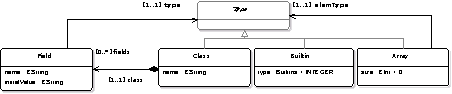
\includegraphics[width=\textwidth]{../postproc/oo-mm}
  \caption{The OO metamodel}
  \label{fig:oo-mm}
\end{figure}

In the remainder of this section, the transformation will be discussed in
details.  FunnyQT contains a feature for generating metamodel-specific APIs
which is used here.  The generated XML and OO APIs are referred to by the
namespace aliases \code|xml| and \code|oo|.  They contain a pair of getter and
setter functions for each attribute (e.g., \code|(xml/name el)| and
\code|(xml/set-name! el val)|), role name accessor functions (e.g.,
\code|(xml/->children el)| or \code|(oo/fields cls)|), and several more.

In FunnyQT, a model-to-model transformation is specified using the
\code|deftransformation| macro.  It receives the name of the transformation
(\code|xml-graph2oo-model|), and a vector defining input models and output
models plus additional parameters.  In this case, there is only one single
input model \code|xml|, one single output model \code|oo|, and no additional
parameters.

\begin{clojurecode*}{numbers=none}
(deftransformation xml-graph2oo-model [[xml] [oo]]
  ...)
\end{clojurecode*}

Inside such a transformation definition, arbitrary many rule and helper
function definitions may occur.  The first rule of the transformation is
\code|element2class| shown in the next listing.

\begin{clojurecode*}{numbers=none}
  (^:top element2class
   :from [e '[:and Element !RootElement]]
   :to   [c (element-name2class (xml/name e))])
\end{clojurecode*}

The \code|^:top| annotation defines this rule as a top-level rule being applied
automatically.  The \code|:from| clause restricts the elements \code|e| this
rule is applicable for to those of metamodel type \code|Element| but not of
type \code|RootElement|.  The reason is that we don't want to create a class
for the \texttt{FIXML} element which is the root element of any FIXML message.

The \code|:to| clause defines which elements should be created for matching
elements.  Usually, it would be specified as \code|:to [x 'SomeClass]| in which
case \code|x| would be a new element of type \code|SomeClass|.  However, in the
current case, there is no one-to-one mapping between XML elements and OO
classes, because the XML model may contain multiple elements with the same tag
name, and there should be exactly one OO class per unique tag name.  Therefore,
the \code|:to| clause delegates the creation of class \code|c| to another rule
\code|element-name2class| providing \code|e|'s tag name as argument.

The semantics of a rule are as follows.  When it is applied to an input element
for which its \code|:from| clause matches, target elements are created
according to its \code|:to| cause.  The mapping from input to output elements
is saved.  When a rule gets applied to an element it has already been applied
to, the elements that have been created by the first call are returned instead
of creating new elements.  That way, calling a rule serves both creation of
target elements as well as resolution of input to output elements in terms of
traceability.

The next rule is \code|element-name2class| which is shown below.

\begin{clojurecode*}{numbers=none}
  (element-name2class
   :from [tag-name]
   :to   [c 'Class {:name tag-name}]
   (doseq [[an at av] (all-attributes tag-name)]
     (attribute2field an at av c))
   (doseq [[tag max-child-no] (all-children tag-name)]
     (children-of-same-tag2field tag max-child-no c))
   (when-let [char-conts (seq (all-character-contents tag-name))]
     (character-contents2field char-conts c)))
\end{clojurecode*}

This rule receives as input a plain string, the \code|tag-name| of an element,
and it creates a \code|Class c| in the target model.  The name of the class
corresponds to the \code|tag-name|.  According to the rule semantics sketched
above and the fact that this rule gets called with the tag name of any element
by \code|element2class|, there will be one target class for every unique tag
name.

Following the \code|:from| and \code|:to| clauses comes the rule's body where
arbitrary code may be written.  Here, three other rules \code|attribute2field|,
\code|children-of-same-tag2field|, and \code|character-contents2field| are
called for all XML attributes, child elements, and character
contents\footnote{The case description doesn't specify if and how XML character
  content should be handled.  However, without them transforming
  \texttt{test3.xml} and \texttt{test4.xml} would lead to classes with no
  fields at all which doesn't make much sense.}  of element \code|e|,
respectively.  These rules and the helpers \code|all-attributes|,
\code|all-children|, and \code|all-character-contents| are skipped in for
brevity, but they follow the same style and mechanics.

The next listing shown the helpers implementing the extension task of
heuristically determining an appropriate field type from XML attribute values.

\begin{clojurecode*}{numbers=none}
  (guess-type [vals]
   (let [ts (set (map #(condp re-matches %
                         #"\d\d\d\d-\d\d-\d\d.*" DATE
                         #"[+-]?\d+\.\d+"        DOUBLE
                         #"[+-]?\d+"             (int-type %)
                         STRING) vals))]
     (get-or-create-builtin-type
      (cond
       (= (count ts) 1)              (first ts)
       (= ts #{DOUBLE INTEGER})      DOUBLE
       (= ts #{DOUBLE LONG})         DOUBLE
       (= ts #{DOUBLE LONG INTEGER}) DOUBLE
       (= ts #{INTEGER LONG})        LONG
       :else                         STRING))))
\end{clojurecode*}

The \code|guess-type| function receives a collection \code|vals| of XML
attribute values.  \code|vals| could either be all character contents of an XML
element, or all attribute values of an attribute that occurs in many XML
elements of the same tag.

Every given value is checked against a regular expression that determines its
type being either a timestamp in ISO 8601 notation, a double value, or an
integer value.  If neither matches, then \code|STRING| is used as its type.  In
case of an integer value, the function \code|int-type| further determines if
the value can be represented as a 32 bit integer, or if a 64 bit long is
needed, or if it is so large that it can only be represented as a string.

The \code|cond| expression picks the type that can be used to represent all
values.  If all values are guessed to be of the very same type, then this type
is chosen.  For multiple numeric types, the respective ``largest'' type is
chosen where \code|INTEGER| < \code|LONG| < \code|DOUBLE|.  Else, we fall back
to \code|STRING|.

The picked type is then passed to the rule \code|get-or-create-builtin-type|
which creates a \code|Builtin| whose \code|type| attribute is set to the picked
type \code|t|.  As a result, the OO model contains at most one \code|Builtin|
element per \code|Builtins| enumeration literal.

The complete \code|xml-graph2oo-model| transformation consists of 6 rules and 7
helpers amounting to 70 lines of code.  The result is an OO model whose field
elements already have the heuristically guessed types, and where
multiple-occuring XML child elements of the same type where compressed to array
fields.  This model can then easily be serialized to code in different
programming languages.


\subsection{OO Model to Code}
\label{sec:oo-model-to-code}

The last step of the overall transformation is to generate code in different
programming languages from the OO model created in the previous step.  In
addition to the core task languages, the FunnyQT solution also generates C code
as an extension.

One crucial benefit of FunnyQT being a Clojure library is that we can simply
use arbitrary other Clojure and Java libraries for our needs.  So for this
task, we use the excellent
\emph{Stencil}\footnote{\url{https://github.com/davidsantiago/stencil}}
library.  Stencil is a Clojure templating library implementing the popular,
lightweight \emph{Mustache}
specification\footnote{\url{http://mustache.github.io/}}.  The idea of Mustache
is that one defines a template file containing placeholders which can be
rendered to a concrete file by providing a map where the keys are the
placeholder names and the values are the text that should be substituted.
There are also placeholders for collections in which case the corresponding
value of the map has to be a collection of maps.

We'll discuss the solution using the template for Java.

\begin{javacode*}{numbers=none}
package {{{pkg-name}}};
{{#imports}}
import {{{imported-class}}};
{{/imports}}

class {{{class-name}}} {
    {{#fields}}
    private {{{field-type}}} {{{field-name}}};
    {{/fields}}

    public {{{class-name}}}() {
	{{#fields}}
	this.{{{field-name}}} = {{{field-value-exp}}};
	{{/fields}}
    }
    // parametrized constructor, getters, and setters elided...
}
\end{javacode*}

So a map to feed to the Stencil templating engine needs to provide they keys
\code|:pkg-name|, \code|:imports|, \code|:class-name|, etc.  The values for the
\code|:imports| and \code|:fields| keys need to be collections of maps
representing one import or field each, e.g., a field is represented as a map
with keys \code|:field-type|, \code|:field-name|, and
\code|:field-value-expression|.

The templates for the other languages use the same keys (although there are
some keys in the C and C++ templates that are only needed by them), so the
essential job of the code generation task is to derive such a map for every
class in our OO model that can then be passed to Stencil's rendering function.

This is done using a FunnyQT polymorphic function \code|to-mustache| whose
definition is given below.

\begin{clojurecode}
(declare-polyfn to-mustache [el lang pkg])
(defpolyfn to-mustache oo.Class [cls lang pkg]
  {:pkg-name pkg
   :imports (get-imports cls lang)
   :class-name (oo/name cls)
   :fields (mark-first-field (map #(to-mustache % lang pkg) (oo/->fields cls)))})
(defpolyfn to-mustache oo.Field [f lang pkg]
  {:field-type (field-type (oo/->type f) lang)
   :field-name (oo/name f)
   :field-value-exp (field-value-exp f lang)
   :plain-field-type (let [t (oo/->type f)]
                       (type-case t
                         'Array (oo/name (oo/->elemType t))
                         'Class (oo/name t)
                         nil))})
\end{clojurecode}

A polymorphic function in FunnyQT is a function that dispatches between several
implementations based on the metamodel type of its first argument.  Thus, you
can view them as a kind of object-oriented method attached to metamodel classes
that may be overridden by subclasses.

Line 1 declares the polymorphic function \code|to-mustache| and defines that it
gets three parameters: an OO model element \code|el|, the target language
\code|lang|, and the package/namespace name \code|pkg| in which the
class/struct should be generated.  Lines 2 to 6 then define an implementation
for elements of the metamodel class \code|Class|, and lines 7-18 define an
implementation for elements of metamodel class \code|Field|.

Both implementations call several helper functions that query the OO model to
compute the relevant values for the map's keys which are skipped for brevity
here.


\section{Evaluation}
\label{sec:evaluation}

The \emph{complexity} according to the evaluation criteria should be measured
as the sum of number of operator occurrences and feature and entity type name
references in the specification expressions.  The FunnyQT solution contains
about 300 expressions (function calls, conditional expressions, etc.), 24
metamodel type references, and 18 property references resulting in a complexity
of 342.  So it is probably quite complex, but most of its complexity is a
result of that it does much more than what was required.

\emph{Accuracy} should measure the degree of syntactical correctness of the
generated code, and the degree of how well the generated code matches the
source FIXML messages.  The FunnyQT solution has a very high accuracy.  The
code is correct for all four languages and compiles without warnings.  It also
matches the source FIXML messages very well.  Especially creating array fields
for XML child elements that occur multiple times is much better than creating
numbered fields.  Also, guessing appropriate types for the fields instead of
always using string improves the usefulness of the generated code.  Finally,
that the transformation can be run on an arbitrarily large sample of FIXML
messages in one go improves the accuracy of the generated classes even more.

Developing the solution has been a on-and-off effort.  All in all, the overall
\emph{development time} can be estimated with about 12 person-hours.

Since FunnyQT's generic \code|xml2xml-graph| transformation uses Java's StAX
API internally, the \emph{fault tolerance} is high.  Documents which are not
well-formed lead to parsing errors.

The \emph{execution time} are good.  For all provided test models, the complete
transformation including parsing XML, transforming the XML model to an OO model
followed by generating code in all four languages took at most 700 milliseconds
on SHARE.  Running the transformation on all provided and five additional FIXML
messages at once took about 1.5 seconds.


Concerning \emph{modularity}, the \code|xml-graph2oo-model| consists of \(r=6\)
rules.  All rules except the top-level rule are called explicitly which gives
\(d=5\).
Thus, its modularity according to the formula \(Mod = 1 - \frac{d}{r}\)
is \(0.1\overline{6}\).
The code generation is implemented with 10 functions that call each other.
Since some functions are recursive and called from different places 12 call
dependencies can be counted.  Thus, the modularity is
\(Mod = 1 - \frac{12}{10} = -0.2\).


With respect to \emph{abstraction level}, FunnyQT model-to-model
transformations like \code|xml-graph2oo-model| are mostly declarative, but
rules may also contain functional/imperative code, and the rules defined here
do so. The code generation is split into declarative templates that express the
contents of the source code files including their formatting, and functions
that derive a map of template placeholder keywords to the values that have to
be filled in for each class.  Those functions are all pure functional, i.e.,
they have no side-effects and are referentially transparent.  Thus, the
abstraction level of the FunnyQT solution is about medium.


\section{Conclusion}
\label{sec:conclusion}

In this paper, the FunnyQT solution to the TTC 2014 FIXML case has been
discussed.  It solves the core task of generating Java, C\#, and C++ code for a
given FIXML message.  The solution also solves the extension tasks of
determining appropriate field types and of generating non-object-oriented C
code.

Furthermore, the FunnyQT solution adds several more features that haven't been
requested like generation of getters and setters, separation of headers and
implementation files for C and C++, the generation of array-valued fields for
XML children of the same tag, and the generation of destructors for C++ and
freeing functions for struct pointers in C.

The generated code in all four languages can be compiled and linked as-is
without warnings or special compiler settings.

Given its amount of features, the solution is quite concise.  The complete
\code|xml-graph2oo-model| transformation consists of 78 lines of code, and the
code generation is implemented in 108 lines of code plus additional 206 lines
of Mustache markup in 12 templates.




\bibliographystyle{alpha}
\bibliography{ttc-fixml}

% \newpage
% \appendix

% \section{Transformation of a Position Report Message}
% \label{sec:posrpt}

% In this section, the stepwise outcomes of transforming a position report
% message (\texttt{test2.xml}) are illustrated.

% The FIXML document itself is printed in Section~\ref{sec:posrpt:xml}.

% Section~\ref{sec:posrpt:xml-graph} shows its representation as TGraph
% conforming to the XML metamodel shown in Figure~\ref{fig:xml-mm}.  This part of
% the overall transformation has been discussed in Section~\ref{sec:xml2model}.

% Section~\ref{sec:posrpt:oo} shows the OO model conforming to the metamodel
% shown in Figure~\ref{fig:oo-mm} which is generated by the
% \code|xml-graph2oo-model| transformation discussed in
% Section~\ref{sec:xml-to-oo}.

% Finally, the sections \ref{sec:posrpt:java}, \ref{sec:posrpt:csharp},
% \ref{sec:posrpt:cpp}, and \ref{sec:posrpt:c} show the source code files for the
% \code|PosRpt| class and the \code|Util| class which contains helpers for the
% data model classes.  For Java and C\#, there is only one source code file for
% the \code|PosRpt| class whereas for C++ and C, the class/struct is declared in
% a header file and its definition is held in a separate implementation file.  It
% should be noted that all source code files are printed here exactly as produced
% by the transformation.  No additional formatting has been done, and they all
% compile without warnings using standard compilers for the languages, i.e.,
% \code|javac| from the OpenJDK project\footnote{\url{http://openjdk.java.net/}}
% for Java, \code|mcs| from the Mono
% project\footnote{\url{http://www.mono-project.com}} for C\#, and
% \code|g++|/\code|gcc| from the GNU Compiler
% Collection\footnote{\url{http://gcc.gnu.org/}} for C++ and C.  However, the C++
% code uses extended initializer lists which are new in the C++11 standard, so a
% \code|-std=c++0x| (or \code|-std=c++11|) has to be added to the \code|g++| call
% in order not to get warnings.


% \subsection{The Position Report as XML document}
% \label{sec:posrpt:xml}

% \xmlfile{../messages/test2.xml}

% \newpage
% \subsection{The Position Report as XML Graph}
% \label{sec:posrpt:xml-graph}
% \begin{center}
%   
\includegraphics[angle=90,height=.95\textheight]{xml-test2}
% \end{center}

% \newpage
% \subsection{The Position Report as OO Model}
% \label{sec:posrpt:oo}
% \begin{center}
%   
\includegraphics[angle=90,height=.95\textheight]{oo-test2}
% \end{center}

% \newpage
% \subsection{The Position Report as Java Class}
% \label{sec:posrpt:java}

% \javafile{../results/java/test2/PosRpt.java}
% \javafile{../results/java/test2/Util.java}

% \newpage
% \subsection{The Position Report as C\# Class}
% \label{sec:posrpt:csharp}

% \csharpfile{../results/csharp/test2/PosRpt.cs}
% \csharpfile{../results/csharp/test2/Util.cs}

% \newpage
% \subsection{The Position Report as C++ Class}
% \label{sec:posrpt:cpp}

% \cppfile{../results/cpp/test2/PosRpt.hpp}
% \cppfile{../results/cpp/test2/PosRpt.cpp}
% \cppfile{../results/cpp/test2/Util.hpp}
% \cppfile{../results/cpp/test2/Util.cpp}

% \newpage
% \subsection{The Position Report as C Struct}
% \label{sec:posrpt:c}

% \cfile{../results/c/test2/PosRpt.h}
% \cfile{../results/c/test2/PosRpt.c}
% \cfile{../results/c/test2/Util.h}
% \cfile{../results/c/test2/Util.c}


\end{document}


%%% Local Variables:
%%% mode: latex
%%% TeX-master: t
%%% TeX-engine: pdflatex-shell-escape
%%% End:
